% Values retained from the independently audited saved-output checkpoint.
\section*{Actual bounded checkpoint}
The final inventory retains 2,149 histories: 999 references, 1,000 null
queries and 150 alternative queries. Of 8,596 planned method outcomes,
7,068 have controlled statistics and 1,528 remain unknown. There are 1,752
histories with all four controlled, 18 partial, three with exceptions and
376 never attempted. One of the partial claimed histories was interrupted with
an uncontrolled final method. Registration is not complete computation.
The two production phases produced 1,639 new terminal records and reused
133 immutable carried records; the claim count was 1,640.

At $\alpha=0.05$, the final accounting is:
\begin{center}
\begin{tabular}{llrrrr}\toprule
Queries & Cell & Reject & Non-reject & Unknown & Rejection bounds\\\midrule
Null ($N=1000$)&$I_{00}$&30&593&377&$[0.030,0.407]$\\
&$I_{10}$&35&588&377&$[0.035,0.412]$\\
&$I_{01}$&31&586&383&$[0.031,0.414]$\\
&$I_{11}$&31&589&380&$[0.031,0.411]$\\\midrule
Alternative ($N=150$)&$I_{00}$&150&0&0&$[1,1]$\\
&$I_{10}$&122&28&0&$[0.8133,0.8133]$\\
&$I_{01}$&150&0&0&$[1,1]$\\
&$I_{11}$&65&82&3&$[0.4333,0.4533]$\\\bottomrule
\end{tabular}
\end{center}
The finite fitting recipe reported here gives 122 rejections out of 150
for $I_{10}$ and 65 rejections, 82 non-rejections and three unknown decisions
for $I_{11}$. These are distinct from the paper's historical counts of
123/150 and 68/150, respectively. A separate source-reported metadata check
matched historical and continuation input identities and case roles; this
compact packet does not reproduce it. No paired historical/continuation
outcome comparison is reported; the counts should not be combined or
interpreted as a paired change in detection.

These are bounds over all planned queries, not confidence intervals or
estimates conditional on successful fitting. Controlled reference counts
are 998, 998, 992 and 997 in cell order; controlled null-query counts are
623, 623, 619 and 620; alternative counts are 150, 150, 150 and 148.
Thus a controlled query can still have an unresolved decision because
reference uncertainty straddles the threshold. Null missingness depends
on history cost, traversal and deadlines; the broad bounds do not establish
empirical 5\% size.

The nuisance-interaction accounting bounds are $[-0.765,0.752]$ under
the null and $[-0.38,-0.36]$ under the alternative. The required full-pair
point mean and MCSE are unavailable for both roles. No survivor-only point
estimate is substituted. On these 150 saved alternative histories, supplying
level and estimating trend gives 150 definite rejections;
estimating both nuisance coordinates is associated with materially fewer
detections. The signed interaction is a procedure contrast, not a causal
effect or proof of physical inhibition.

\subsection*{Completed descriptive resampling}
All 2,000 declared replicates completed, using one shared reference plan
across the four cells and both roles, and separate paired query plans by
role. Lower and upper accounting endpoints are summarized separately with
linear/type-7 quantiles. For the alternative $I_{11}$ cell, the 2.5\%, median
and 97.5\% quantiles of the lower endpoint are $(0.3800,0.4333,0.4667)$
for bank-only resampling and $(0.3400,0.4333,0.5200)$ when paired queries
are also resampled. The corresponding upper-endpoint quantiles are
$(0.4067,0.4533,0.4800)$ and $(0.3600,0.4533,0.5400)$.
These summarize sensitivity of incomplete accounting, not certified coverage.
All 120 endpoint quantiles and counts of every replicate status are retained
in the JSON/CSV tables; individual statuses remain in the saved chunk JSON.
No unresolved replicate is discarded. In the alternative
paired-query mode, 126 replicates have a resolved point interaction and
1,874 remain unresolved. This does not resolve the original full-pair point.

\subsection*{Posthoc accounting of the continuation pilot}
This subsection concerns the earlier 25-query pilot of this continuation,
not the paper's separate $\eta$-planning experiment (6/25 versus 11/25).
After inspecting the aggregate calibration, a separate saved-evidence check
fixed the original 25 alternative IDs and compared their unchanged carried
scores under the old and expanded reference banks. This was descriptive
posthoc accounting: no fit, rank plan or history was regenerated.
For $I_{10}$, the original cohort changed from $(6,11,8)$ to $(19,6,0)$
in reject/non-reject/unknown counts. The remaining 125 alternatives gave
$(103,22,0)$ under the same final bank. For $I_{11}$, the original cohort
changed from $(6,17,2)$ to $(8,17,0)$ and the remaining cohort gave
$(57,65,3)$. Both cohorts have all rejections in $I_{00}$ and $I_{01}$.
The same 25 fitted scores yield different decisions under the new reference
calibration. This comparison does not isolate bank size from reference
composition, rank resolution or missingness. Neither
this comparison nor the additional query cohort establishes population
causality, independent validation or nominal test size.

\begin{figure}[p]
\centering
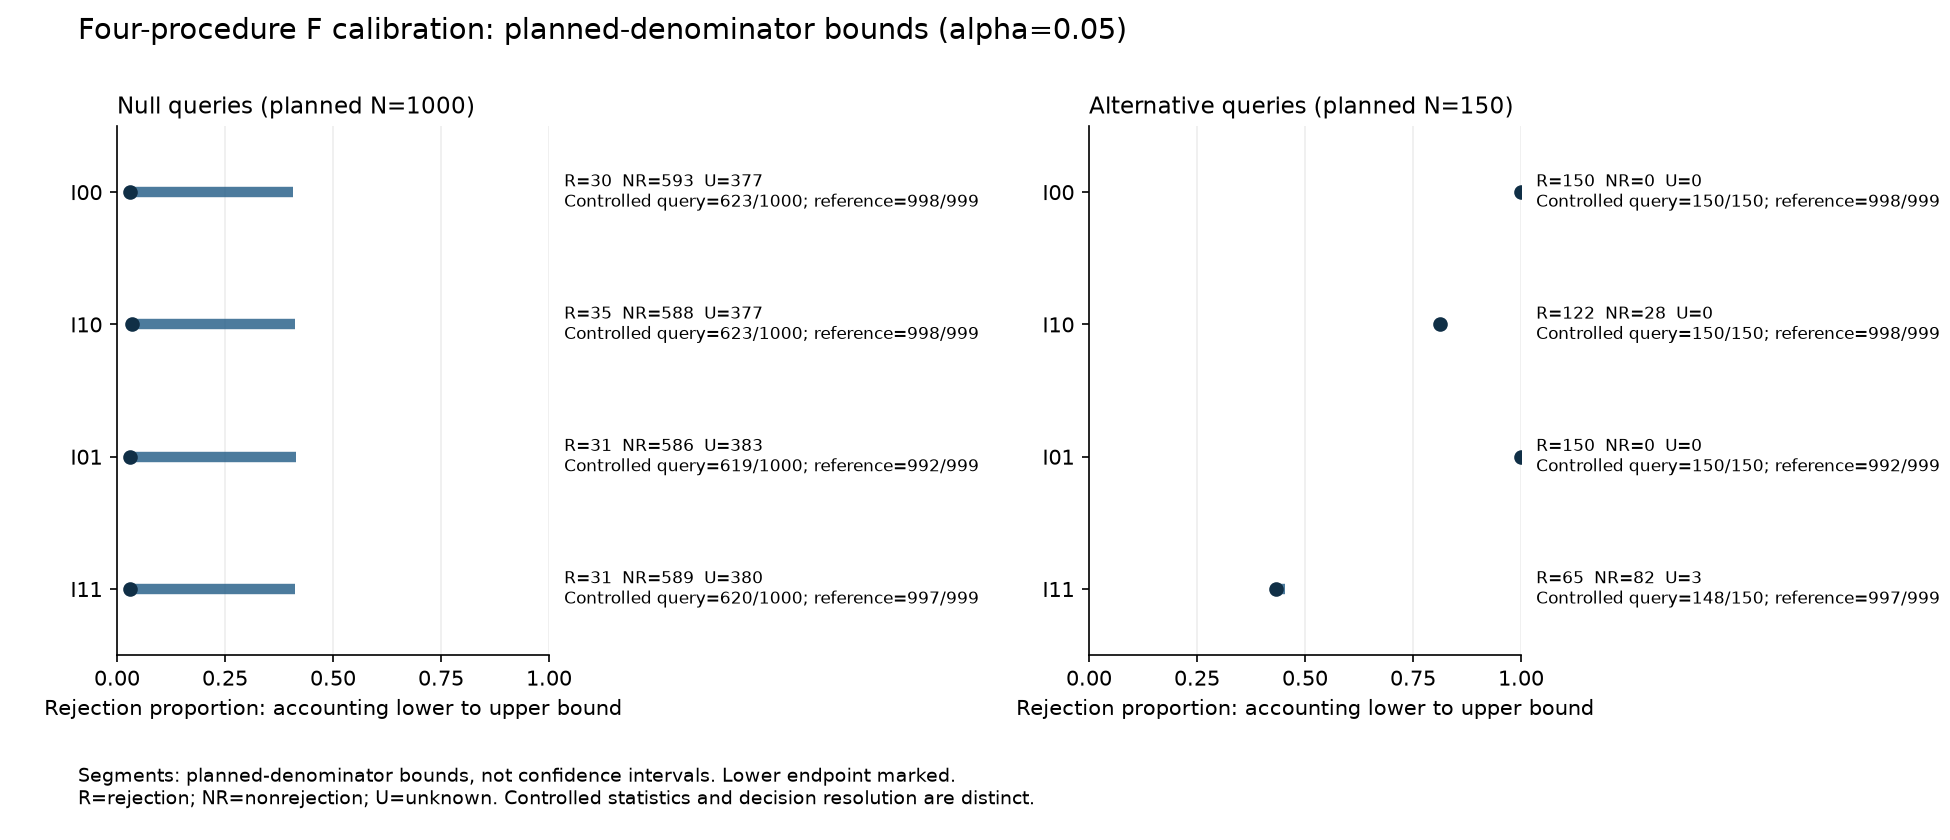
\includegraphics[width=\textwidth]{figures/F04_calibration01/F04_planned_denominator_bounds.png}
\caption{Actual final calibration on the full planned denominators.
Segments span definite rejection through rejection plus unresolved outcomes;
they are accounting bounds. The figure retains unknowns and controlled
query/reference counts.}
\end{figure}

\subsection*{Next decision}
The continuation stops at this incomplete evidence checkpoint. Incomplete
null coverage prevents a calibrated-size conclusion. Reopening the study
would first require a bounded demonstration of a substantially cheaper,
numerically valid recovery procedure, with consistent rules across roles
and cells. Old failures would remain preserved, and any reference-bank
change would require recalibration of the entire contrast. No such recovery,
cache change, fresh bank or wider scientific campaign accompanies this
manuscript revision.
